% ============================================================
%  Digital Twin-Driven Flood Evacuation System Using AI Optimization
%  IEEE Journal Format — IEEEtran
%  M.S. Ramaiah Institute of Technology, CSP81 Project
% ============================================================

\documentclass[journal]{IEEEtran}

% ---- Packages ----
\usepackage[utf8]{inputenc}
\usepackage[T1]{fontenc}
\usepackage{amsmath}
\usepackage{amssymb}
\usepackage{graphicx}
\usepackage{booktabs}
\usepackage{multirow}
\usepackage{array}
\usepackage{float}
\usepackage{url}
\usepackage{hyperref}
\usepackage{algorithm}
\usepackage{algorithmic}
\usepackage{xcolor}
\usepackage{cite}

\hypersetup{
    colorlinks=true,
    linkcolor=blue,
    citecolor=blue,
    urlcolor=blue
}

% ============================================================
\begin{document}

\title{Digital Twin-Driven Flood Evacuation System Using AI Optimization}

\author{
  \IEEEauthorblockN{Aditri B Ray\textsuperscript{1},\; Anisha Ajit\textsuperscript{1},\; Diya D Shah\textsuperscript{1}}\\
  \IEEEauthorblockA{\textsuperscript{1}Department of Computer Science and Engineering,\\
  M.S. Ramaiah Institute of Technology (Autonomous, Affiliated to VTU),\\
  Bengaluru, Karnataka, India}\\
  \IEEEauthorblockA{\textit{Guide:} Dr. Mallegowda M., M.S. Ramaiah Institute of Technology}
}

\maketitle

% ============================================================
\begin{abstract}
Urban flooding causes thousands of fatalities and displaces millions annually, yet most
municipal evacuation systems rely on static, pre-computed route tables that cannot adapt
to real-time flood dynamics. This paper presents \textit{UrbanFloodReact}, a digital twin
platform for adaptive flood evacuation planning deployed over Bengaluru, India's
350$+$ administrative sub-units (hoblis). The system couples a simplified Storm Water
Management Model (SWMM) hydraulic propagation engine with three metaheuristic optimization
algorithms (Genetic Algorithm, Ant Colony Optimization, and Particle Swarm Optimization)
operating on OpenStreetMap-derived road network graphs. Real-time traffic congestion
(TomTom API) and precipitation data (Open-Meteo API) are integrated into flood-weighted
edge costs, producing routes that reflect live road conditions. A Generative AI advisory
layer, structured through the Model Context Protocol (MCP) and grounded via a
SentinelBridge state-synchronization mechanism, delivers multi-persona decision support
to emergency coordinators without displacing human authority. All three optimizers share a
unified base planner providing identical Dijkstra preprocessing, a common fitness function,
and a shared capacity repair operator. Evaluation across 3-run stability trials at 120 mm
rainfall over a representative Bengaluru hobli shows ACO achieves the lowest mean
evacuation cost (fitness: 583,600 vs.\ GA's 588,500) with 99.79\% stochastic stability,
PSO converges fastest (5--10 iterations), and GA generates the most route diversity
($>$30\% unique assignments). Results are streamed live via Server-Sent Events (SSE),
enabling frame-by-frame flood visualization for emergency management personnel.
\end{abstract}

\begin{IEEEkeywords}
digital twin, flood evacuation, metaheuristic optimization, generative AI, model context
protocol, urban computing, disaster informatics, Bengaluru
\end{IEEEkeywords}

% ── Bilingual Abstract (zh-TW) ───────────────────────────────────────────────
% NOTE: Chinese characters require XeLaTeX + xeCJK package.
% To enable: (1) switch compiler to XeLaTeX in Overleaf (Menu → Compiler),
%            (2) add to preamble: \usepackage{xeCJK}
%            (3) uncomment the block below.
%
%\begin{abstract}
%城市洪災每年造成大量傷亡並迫使數百萬人流離失所，而現行疏散系統多依賴靜態路由方案，
%無法因應即時洪災動態。本研究提出 \textit{UrbanFloodReact}，一套以數位孿生技術為核心的
%洪災疏散規劃平台，部署於印度班加羅爾（Bengaluru）逾350個行政次分區（Hobli）。系統整合
%簡化式暴雨水管理模型液壓傳播引擎與三種元啟發式最佳化演算法（遺傳演算法、蟻群演算法、
%粒子群演算法），結合即時交通與降雨數據動態調整洪災加權路徑邊際成本。生成式人工智慧諮詢層
%透過模型上下文協議（MCP）與 SentinelBridge 狀態同步機制，向緊急協調人員提供多角色決策支援，
%同時防止大型語言模型產生幻覺。三種演算法共享統一基礎規劃器，確保演算法比較的公正性。
%實驗於120 mm降雨情境下進行三次穩定性測試：蟻群演算法達到最低均值適應度（583,600）且
%隨機穩定性達99.79\%，粒子群演算法收斂最快（5至10次迭代），遺傳演算法則產生最高路徑
%多樣性（28至35\%）。所有結果透過伺服器推送事件即時串流，提供逐幀洪災視覺化呈現。
%\end{abstract}
%
%\begin{IEEEkeywords}
%數位孿生、洪災疏散、元啟發式最佳化、生成式人工智慧、模型上下文協議、都市運算、緊急管理
%\end{IEEEkeywords}

% ============================================================
\section{Introduction}
\label{sec:intro}

Floods are the most frequent and costliest natural disaster category worldwide, with urban
areas bearing a disproportionate share of their impact \cite{anik2025evolution}. Bengaluru,
India's third-largest metropolitan area, exemplifies this vulnerability: the city's lake
network has contracted sharply over recent decades as urban encroachment replaced natural
water retention areas, leaving road networks as the primary flood pathway during the
southwest monsoon season \cite{mujumdar2021bengaluru}. The Integrated Urban Flood Management
programme for Indian cities \cite{mujumdar2017integrated} identified real-time decision
support and community-scale evacuation coordination as critical gaps in the national response
framework.

Emergency evacuation during a flood event demands decisions that compound in complexity every
minute: Which roads are passable? Which shelters have remaining capacity? Where are the
bottlenecks forming? Traditional evacuation management systems resolve these questions using
static plans prepared days or weeks before an event. When flood conditions deviate from
anticipated patterns — as they routinely do — field coordinators are left without decision
support adapted to the actual state of the city.

The concept of a \textit{digital twin} offers a principled response to this gap.
Grieves~\cite{grieves2014} formalized the digital twin as a virtual replica of a physical
system that maintains bidirectional synchronization with its real-world counterpart. In urban
emergency management, a digital twin maps the physical city — its road network, population
distribution, shelter locations, and hydraulic state — into a computational model that can be
queried, simulated, and optimized in real time \cite{mandal2025cityscale, riaz2023climate,
zhou2024framework}.

\subsection{Research Gaps}

A review of the literature identifies five specific gaps that motivate the present work:

\begin{enumerate}
  \item \textbf{Prediction-Action Disconnect.} Existing flood prediction systems and
  evacuation routing modules are developed and deployed independently, creating a critical
  latency between hazard detection and route re-computation \cite{gupta2025ai,
  anik2025evolution}. No unified framework continuously feeds physics-derived flood depths
  into live optimizer edge weights.

  \item \textbf{Limited Multi-Algorithm Routing in Digital Twins.} Digital twin platforms for
  flood management \cite{zhou2025rainfall, mandal2025cityscale, prihatmanto2025digitaltwin}
  typically adopt a single routing or optimization strategy. Head-to-head comparison of GA,
  ACO, and PSO under identical problem instances — necessary for informed operational
  deployment — is absent in the current literature \cite{yin2025overview, li2025metaheuristic}.

  \item \textbf{Computational Scalability Gap.} Most metaheuristic evacuation studies operate
  on small synthetic networks \cite{nirwana2024intelligent, li2024evacuation}. City-scale
  deployment over 350$+$ heterogeneous hobli graphs, each requiring Dijkstra preprocessing
  and capacity-aware search, has not been demonstrated.

  \item \textbf{Lack of GenAI Decision Explanation.} Human-centered flood management
  frameworks \cite{alizadeh2023humancentered, behrooz2024adaptive} surface route
  recommendations without natural-language explanation, leaving coordinators unable to
  interrogate the reasoning behind suggested actions. LLM-based explanation grounded in live
  simulation state is absent from existing platforms.

  \item \textbf{Absence of Unified Congestion-Aware Digital Twin Architecture.}
  Congestion-aware flood evacuation \cite{wang2024congestion} and multi-agency coordination
  \cite{chen2025evacuation} are studied separately. A single unified architecture integrating
  real-time traffic (TomTom), flood simulation (SWMM-simplified), metaheuristic optimization,
  and GenAI advisory — operating over a live OSMnx city graph — has not been reported.
\end{enumerate}

\subsection{Contributions}

This paper describes \textit{UrbanFloodReact}, a full-stack digital twin platform for flood
evacuation planning that directly addresses each gap above. The system makes five technical
contributions:

\begin{enumerate}
  \item A physics-based flood propagation model (Gap 1), implemented as a simplified SWMM
  engine on an OSMnx road graph \cite{boeing2017}, that generates spatially distributed
  flood depth estimates used to penalize routing edges in real time.

  \item A unified evacuation optimization framework (Gap 2), running GA, ACO, and PSO over a
  shared fitness function, Dijkstra preprocessing, and capacity repair operator — enabling
  rigorous head-to-head comparison on identical problem instances over Bengaluru's OSMnx graph.

  \item A scalable deployment architecture (Gap 3) covering 350$+$ hoblis with lazy graph
  loading, MongoDB caching, and shared Dijkstra matrix precomputation achieving a $9\times$
  speedup during multi-algorithm stability trials.

  \item A Generative AI advisory architecture (Gap 4), built on the Model Context Protocol
  \cite{anthropic2024mcp} with a three-tier LLM reliability stack (Gemini 2.5 Flash
  \cite{gemini2023} / Groq / Ollama), delivering persona-differentiated decision support
  grounded in live simulation state via the SentinelBridge state synchronization layer.

  \item A congestion-aware live streaming architecture (Gap 5) using TomTom Traffic API
  \cite{tomtom2024} to modulate edge costs and Server-Sent Events (SSE) to render flood
  propagation and routes frame-by-frame in the browser.
\end{enumerate}

The remainder of the paper is organized as follows. Section~\ref{sec:related} surveys related
work. Section~\ref{sec:arch} describes the system architecture. Sections~\ref{sec:flood} and
\ref{sec:formulation} present the flood model and evacuation formulation respectively.
Section~\ref{sec:algorithms} details the three algorithm implementations. Section~\ref{sec:genai}
describes the GenAI advisory layer. Section~\ref{sec:eval} reports experimental results.
Sections~\ref{sec:discussion} and \ref{sec:conclusion} discuss findings and conclude.

% ============================================================
\section{Related Work}
\label{sec:related}

\subsection{Flood Prediction and Urban Hydraulic Modeling}

Urban flood prediction has evolved from process-based hydrological models toward machine
learning and data-driven approaches. Anik et al.\ \cite{anik2025evolution} survey this
transition, noting that convolutional and recurrent neural networks now outperform
physics-based models on short-term flood depth forecasting but lack interpretability for
emergency response. Gupta et al.\ \cite{gupta2025ai} provide a comprehensive review of AI
for flood risk management, identifying the disconnect between prediction capability and
actionable response as the defining open problem. At the city scale, Mujumdar et al.\
\cite{mujumdar2021bengaluru} developed an urban flood model specifically for Bengaluru,
demonstrating that simplified hydraulic models calibrated to local drainage infrastructure
are feasible and computationally tractable for monsoon planning. The present work builds on
this Bengaluru-specific knowledge base, adapting simplified SWMM head propagation for
real-time computation over OSMnx road graphs \cite{rossman2010}.

\subsection{Evacuation Route Optimization}

Evacuation routing has been cast as a network flow, vehicle routing, and multi-objective
optimization problem, with metaheuristic algorithms gaining prominence for city-scale
instances where exact methods are intractable. Li et al.\ \cite{li2024evacuation} proposed
a novel emergency evacuation route optimization model integrating dynamic flood conditions;
Yin et al.\ \cite{yin2025overview} survey evacuation planning models and identify
multi-shelter, capacity-constrained routing as an underexplored regime. Nirwana et al.\
\cite{nirwana2024intelligent} applied PSO-based intelligent optimization to natural disaster
evacuation, demonstrating feasibility but without comparison against competing metaheuristics.
Xu and Zhang \cite{xu2024aco} integrated ACO with agent-based simulation for urban flood
rescue routing with multi-center vehicle routing, while Li et al.\ \cite{li2025metaheuristic}
compared metaheuristic algorithms on a York flood case study. Basheer et al.\
\cite{basheer2023priority} combined GIS with fuzzy AHP for priority-based evacuation
simulation. Behrooz and Ilbeigi \cite{behrooz2024adaptive} introduced adaptive routing with
directional road control. The distinguishing feature of UrbanFloodReact is a \textit{unified
base planner} that enforces identical Dijkstra preprocessing, fitness function, and capacity
repair across GA, ACO, and PSO — ensuring that observed performance differences are
attributable to algorithmic behavior, not implementation inconsistencies.

\subsection{Digital Twins for Urban Emergency Management}

The digital twin concept \cite{grieves2014} has been extended to urban flood management
through several recent frameworks. Zhou et al.\ \cite{zhou2025rainfall} proposed a
framework incorporating real-time rainfall data into a flooding digital twin, emphasizing
the importance of sensor fusion for hydraulic state estimation. Zhou et al.\
\cite{zhou2024framework} defined an urban flooding digital twin system framework with
modular simulation, monitoring, and decision support components. Mandal et al.\
\cite{mandal2025cityscale} demonstrated a city-scale digital twin for flood impact analysis
integrating urban infrastructure and real-time data analytics. Riaz et al.\
\cite{riaz2023climate} explored digital twin technology combined with 3D city modelling and
early warning systems for climate resilience. Prihatmanto et al.\
\cite{prihatmanto2025digitaltwin} demonstrated a digital twin city framework specifically
targeting flood evacuation systems. Wang et al.\ \cite{wang2024congestion} addressed
congestion risks in flood-disrupted transportation networks through topological analysis.
Chen et al.\ \cite{chen2025evacuation} presented a large-scale real-time evacuation model
with a coupled agent-based multi-model framework. Human-centered aspects are addressed by
Alizadeh et al.\ \cite{alizadeh2023humancentered}, who augmented flood gauge data with
crowdsourced street photos for intelligent routing. UrbanFloodReact unifies flood physics,
optimization, congestion data, and AI advisory into a single operational loop — the
unified architecture gap identified in existing platforms.

\subsection{Generative AI in Disaster Response}

Large language models have demonstrated potential as advisory interfaces in high-stakes
domains when structured tool access constrains hallucination pathways. Zhang et al.\
\cite{zhang2023drl} applied deep reinforcement learning to uncertain urban flood path
planning, illustrating the value of learning-based decision support. The Gemini family of
multimodal models \cite{gemini2023} introduced function-calling capabilities enabling LLMs
to retrieve structured state rather than generating it from parametric memory. The Model
Context Protocol (MCP) \cite{anthropic2024mcp} formalizes this pattern by defining typed
tool schemas that LLMs invoke against live data servers. UrbanFloodReact adopts MCP as the
interface between its GenAI advisory layer and the live simulation state, ensuring that
AI-generated recommendations are grounded in current flood model output through a dedicated
state synchronization layer (SentinelBridge).

% ============================================================
\section{System Architecture}
\label{sec:arch}

\subsection{Overview}

UrbanFloodReact is a full-stack web application composed of a React 19 frontend and a
Python 3.12 FastAPI backend. The frontend communicates with the backend over REST and
Server-Sent Events (SSE). Three external services — TomTom Traffic API \cite{tomtom2024},
Open-Meteo weather API \cite{zippenfenig2023}, and MongoDB — provide traffic data,
real-time precipitation, and graph caching respectively. Fig.~\ref{fig:arch} illustrates
the system architecture.

\begin{figure}[H]
  \centering
  \fbox{\parbox{0.85\linewidth}{\centering
    \small\textit{System architecture diagram: React 19 Frontend $\leftrightarrow$ FastAPI
    Backend (Flood Simulator $\|$ GA/ACO/PSO Planners $\|$ GenAI Layer $\|$ MCP Servers
    $\|$ SentinelBridge) $\leftrightarrow$ TomTom / Open-Meteo / MongoDB}
  }}
  \caption{High-level architecture of UrbanFloodReact. Arrows indicate data flow direction;
  double arrows indicate bidirectional SSE streams. SentinelBridge synchronizes physics
  engine state to the GenAI layer via disk-backed \texttt{mcp\_state.json}.}
  \label{fig:arch}
\end{figure}

\subsection{Backend Modules}

The FastAPI backend (Python 3.12) exposes 18 HTTP endpoints and three SSE generator
coroutines. The main modules are:

\begin{itemize}
  \item \textbf{Flood Simulator} (\texttt{flood\_simulator.py}, 12.6 KB) — SWMM-simplified
  hydraulic propagation on the road graph with instant and progressive rainfall modes.

  \item \textbf{Base Planner} (\texttt{base\_planner.py}, 313 LOC) — Dijkstra preprocessing,
  shared fitness function, greedy seed, and capacity repair operator shared by all three
  algorithm implementations.

  \item \textbf{Evacuation Planners} (\texttt{genetic\_algorithm/core.py},
  \texttt{aco/core.py}, \texttt{pso/core.py}) — per-algorithm optimization loops inheriting
  from the unified base planner.

  \item \textbf{Region Manager} (\texttt{region\_manager.py}, 61.2 KB) — OSMnx graph
  download, hobli hierarchy management, and MongoDB caching of directed multigraphs.

  \item \textbf{SentinelBridge} (\texttt{sentinel\_bridge.py}) — disk-backed state
  synchronization class that writes the current simulation output to \texttt{mcp\_state.json}
  after each optimization cycle, enabling MCP servers to serve live data without
  cross-process shared memory.

  \item \textbf{GenAI Layer} (\texttt{genai/expert\_panel.py}, 977 LOC;
  \texttt{genai/app\_copilot.py}, 609 LOC) — streaming expert advisory and
  function-calling copilot backed by the three-tier LLM stack.

  \item \textbf{MCP Servers} — four Model Context Protocol servers exposing typed tools
  for LLM reasoning, grounded in SentinelBridge state (Section~\ref{sec:genai}).
\end{itemize}

\subsection{Security: Authentication and Access Control}

The API enforces Role-Based Access Control (RBAC) via JSON Web Tokens (JWT). Three roles
are defined: \texttt{coordinator} (full read/write access to simulation and advisory
endpoints), \texttt{viewer} (read-only access to simulation state and maps), and
\texttt{admin} (user management, configuration endpoints). All JWT tokens include an
expiry claim enforced server-side; expired tokens are rejected with HTTP 401. Simulation
trigger endpoints require at minimum the \texttt{coordinator} role, preventing unauthorized
initiation of computationally expensive optimization runs.

\subsection{Graceful Degradation}

The system is designed to degrade gracefully when external services are unavailable:
\begin{itemize}
  \item \textbf{TomTom failure} — traffic multiplier defaults to 1.0 (free-flow assumption);
  flood-weighted Dijkstra proceeds without congestion adjustment. A warning banner is shown
  in the frontend.
  \item \textbf{Open-Meteo failure} — the user-specified rainfall value is used directly;
  live precipitation data is not fetched.
  \item \textbf{MongoDB unavailable} — OSMnx downloads the graph on demand; caching is
  skipped with a console warning.
  \item \textbf{GenAI tier exhaustion} — if all three LLM tiers fail, the advisory panel
  displays a structured fallback message using the last available simulation metrics.
\end{itemize}

\subsection{Geographic Scope}

The system covers Bengaluru Urban and Rural regions across more than 350 hoblis — the
lowest-level administrative sub-units within the Bruhat Bengaluru Mahanagara Palike (BBMP)
jurisdiction. Road graphs are lazily loaded from OpenStreetMap \cite{osm2017} via OSMnx
\cite{boeing2017} and cached in MongoDB to avoid repeated network requests. Each hobli
graph is a directed multigraph $G = (V, E)$ with node-level elevation (SRTM), population
(2011 Bengaluru Census $+$ 15\% growth projection), and water depth attributes, and
edge-level length, travel time, and flow efficiency attributes.

\subsection{Frontend}

The React 19 frontend uses MapLibre GL for WebGL-accelerated map rendering on CartoDB
Positron basemap tiles. Key components include a real-time flood layer rendering three
severity zones (shallow, moderate, deep), an evacuation route layer with citizen and shelter
pins, an algorithm performance dashboard, and the AI Expert Panel interface. All simulation
results arrive via SSE streams and are rendered progressively as each event fires.

% ============================================================
\section{Flood Physics Model}
\label{sec:flood}

\subsection{Model Description}

The flood simulator implements a graph-based simplified SWMM approach using hydraulic head
propagation \cite{rossman2010}. Unlike full SWMM, which solves the Saint-Venant equations
across a pipe network with subcatchment geometry, the simplified model propagates water
depth node-to-node on the OSMnx road graph, treating each intersection as a storage node.
This approximation is appropriate for real-time operation: a complete simulation over a
hobli graph finishes in under two seconds on commodity hardware, compared to minutes for
full SWMM with equivalent spatial coverage \cite{mujumdar2021bengaluru}.

\subsection{Initialization Modes}

The simulator supports two rainfall initialization strategies:

\textbf{Instant Mode (Flash Flood):} Water is loaded directly at drainage and water body
nodes at simulation start:
\begin{align}
  h_{\text{drain}}(n) &= 25 \times r_{\text{mm}} \label{eq:init_drain} \\
  h_{\text{lake}}(n)  &= 100 \times r_{\text{mm}} \label{eq:init_lake}
\end{align}
where $r_{\text{mm}}$ is total rainfall in millimetres. This models drain overflow or
flash flood scenarios.

\textbf{Progressive Mode (Gradual Accumulation):} Rainfall is distributed evenly across
simulation steps:
\begin{equation}
  \Delta w(n, t) = \frac{r_{\text{mm}}}{\tau}
  \label{eq:progressive}
\end{equation}
where $\tau$ is the number of simulation steps. Progressive mode reproduces the
spatial spread characteristic of sustained monsoon rainfall.

\subsection{Propagation Algorithm}

At each time step $t$, for every node $n \in V$, propagation proceeds as follows.

\textbf{Hydraulic head:}
\begin{equation}
  \text{head}(n) = \text{elev}(n) + w(n, t)
  \label{eq:head}
\end{equation}

\textbf{Downhill flow identification:}
\begin{equation}
  \mathcal{L}(n) = \{ nb \in \mathcal{N}(n) \mid \text{head}(nb) < \text{head}(n) \}
  \label{eq:lower}
\end{equation}

\textbf{Proportional flow distribution:} For each $nb \in \mathcal{L}(n)$:
\begin{equation}
  f(n, nb) = \frac{\Delta h(n, nb)}{\sum_{nb' \in \mathcal{L}(n)} \Delta h(n, nb')}
  \label{eq:flow_frac}
\end{equation}
where $\Delta h(n, nb) = \text{head}(n) - \text{head}(nb)$.

\textbf{Slope amplification factor:}
\begin{equation}
  s(n, nb) = 1 + \min\!\left(\frac{|\text{elev}(n) - \text{elev}(nb)|}{10},\ 2.0\right)
  \label{eq:slope}
\end{equation}

\textbf{Outflow per neighbor:}
\begin{equation}
  q(n, nb) = w(n,t) \cdot \delta \cdot f(n, nb) \cdot s(n, nb) \cdot \eta(n, nb)
  \label{eq:outflow}
\end{equation}
where $\delta = 0.5$ is the decay factor (fraction of available water that flows per step)
and $\eta(n, nb) \in [0,1]$ is an edge flow efficiency attribute serving as a proxy for
Manning's roughness coefficient \cite{rossman2010}.

\textbf{Conservation constraint:}
\begin{equation}
  \sum_{nb \in \mathcal{L}(n)} q(n, nb) \leq w(n, t)
  \label{eq:conservation}
\end{equation}

Nodes with $w(n,t) < 0.005$ m are skipped as sources in that step to prevent numerical
noise from propagating through dry regions.

\subsection{Risk Classification}

Four risk levels are assigned by absolute depth threshold:

\begin{table}[H]
  \centering
  \caption{Flood Risk Classification Thresholds}
  \label{tab:risk}
  \begin{tabular}{@{}llll@{}}
    \toprule
    \textbf{Level} & \textbf{Depth (m)} & \textbf{Map Color} & \textbf{Operational Meaning} \\
    \midrule
    Safe     & $< 0.15$          & ---    & No significant flooding        \\
    Shallow  & $0.15$--$0.20$    & Green  & Minor flooding, passable       \\
    Moderate & $0.20$--$0.50$    & Yellow & Vehicle difficulty; caution    \\
    Deep     & $> 0.50$          & Red    & Impassable; evacuation trigger \\
    \bottomrule
  \end{tabular}
\end{table}

A node $n$ is designated \textit{at-risk} when $\max_t w(n,t) \geq 0.20\,\text{m}$ and
$\text{pop}(n) > 0$ (the Moderate-or-above threshold, corresponding to vehicle difficulty).
Nodes in the Shallow zone ($0.15$--$0.20$ m) are considered passable and are not treated
as evacuation sources. The at-risk node set $R \subset V$ is the input to the evacuation
planner.

% ============================================================
\section{Evacuation Planning Formulation}
\label{sec:formulation}

\subsection{Problem Definition}

Given a directed road graph $G = (V, E)$ produced by the flood simulator, the evacuation
planner solves the following assignment problem:

\begin{itemize}
  \item \textbf{At-risk nodes:} $R \subset V$ with population $\text{pop}(r)$ for each
  $r \in R$.
  \item \textbf{Shelters:} $S \subset V$ with capacity $\text{cap}(s)$ for each $s \in S$.
  \item \textbf{Pre-computed matrices:} $D[r,s]$ (flood-weighted shortest-path distance) and
  $T[r,s]$ (flood-weighted travel time) from Dijkstra's algorithm \cite{dijkstra1959} run
  outward from each shelter node.
\end{itemize}

The goal is to find a chromosome (assignment) $C: R \to S$ that minimizes total evacuation
cost while satisfying shelter capacity constraints.

\subsection{Flood-Weighted Edge Cost}

Each edge $(u, v)$ receives a modified traversal cost that penalizes flooded road segments:
\begin{equation}
  w_{\text{flood}}(u,v) = \ell(u,v) \cdot \left(1 + 5 \cdot \bar{d}(u,v)\right)
  \label{eq:flood_weight}
\end{equation}
where $\ell(u,v)$ is the edge length in metres and
$\bar{d}(u,v) = (w(u) + w(v)) / 2$ is the mean water depth at the edge endpoints.
The coefficient 5 reflects the operational observation that a road with 1 m of standing
water requires approximately six times the traversal time or effort of a dry road
\cite{behrooz2024adaptive}.

When TomTom live traffic data is available \cite{tomtom2024}, the edge cost is further
multiplied by a congestion factor:
\begin{equation}
  w_{\text{traffic}}(u,v) = w_{\text{flood}}(u,v) \cdot
  \min\!\left(5.0,\ \frac{t_{\text{current}}(u,v)}{t_{\text{free}}(u,v)}\right)
  \label{eq:traffic_weight}
\end{equation}
capping the traffic multiplier at $5\times$ to prevent numerical instability on severely
congested segments, consistent with approaches in \cite{wang2024congestion}.

\subsection{Fitness Function}

The shared fitness function $F(C)$, minimized by all three algorithms, is:
\begin{align}
  F(C) &= \underbrace{\sum_{r \in R} D[r,\, C(r)] \cdot \text{pop}(r)}_{\text{distance cost}}
         + \underbrace{0.5 \sum_{r \in R} T[r,\, C(r)] \cdot \text{pop}(r)}_{\text{time cost}}
         \notag \\
       &\quad + \underbrace{\sum_{s \in S} \max\!\bigl(0,\, \ell_s - \text{cap}(s)\bigr)^2
                           \cdot 10^5}_{\text{capacity penalty}}
         + \sum_{r \in R} \rho(r,\, C(r)) \cdot \text{pop}(r)
         \notag \\
       &\quad + 10^6 \cdot P_{\text{unassigned}}
         \label{eq:fitness}
\end{align}
where $\ell_s = \sum_{r: C(r)=s} \text{pop}(r)$ is the total population load at shelter
$s$, $\rho(r, s)$ is a terrain penalty that discourages routing toward shelters
significantly lower in elevation than the source node (elevation drop $> 50\,\text{m}$
incurs a per-person penalty of 500), and $P_{\text{unassigned}}$ is the count of citizens
with no valid shelter assignment ($C(r) = -1$).

The quadratic capacity penalty $(10^5 \times \text{overflow}^2)$ is chosen to strongly
discourage shelter overfilling while remaining smooth for gradient-free optimizers
\cite{li2024evacuation}.

\subsection{Greedy Initialization}

All three algorithms seed their initial population/swarm with a common greedy chromosome:

\begin{algorithm}[H]
  \caption{Greedy Seed Chromosome Construction}
  \label{alg:greedy}
  \begin{algorithmic}[1]
    \STATE Sort $R$ by $\text{pop}(r)$ descending
    \FOR{each $r \in R$ (in sorted order)}
      \STATE $s^* \leftarrow \arg\min_{s \in S,\ \text{rem}(s) \geq \text{pop}(r)} D[r, s]$
      \IF{$s^*$ exists}
        \STATE $C(r) \leftarrow s^*$; update $\text{rem}(s^*)$
      \ELSE
        \STATE $C(r) \leftarrow -1$
      \ENDIF
    \ENDFOR
  \end{algorithmic}
\end{algorithm}

This greedy seed is inserted as one individual in 80\% of the initial population and used
as the starting point for PSO particles. The remaining 20\% (GA, PSO) or all particles
beyond the seed (PSO) are initialized with capacity-aware random assignments.

\subsection{Capacity Repair Operator}

After any modification to a chromosome (crossover, mutation, or velocity update), a repair
operator enforces shelter capacity feasibility:

\begin{algorithm}[H]
  \caption{Capacity Repair Operator}
  \label{alg:repair}
  \begin{algorithmic}[1]
    \FOR{each shelter $s$ with $\ell_s > \text{cap}(s)$}
      \STATE Sort over-assigned nodes by $D[r, s]$ descending (worst fit first)
      \FOR{each over-assigned node $r$}
        \STATE candidates $\leftarrow$ shelters with $\text{rem}(s') \geq \text{pop}(r)$,
               sorted by $D[r, s']$
        \IF{candidates non-empty}
          \STATE $C(r) \leftarrow \arg\min$ candidates
        \ELSE
          \STATE $C(r) \leftarrow -1$
        \ENDIF
      \ENDFOR
    \ENDFOR
  \end{algorithmic}
\end{algorithm}

Sharing this repair operator across GA, ACO, and PSO ensures that capacity feasibility is
enforced identically, preventing any single algorithm from achieving a fitness advantage
through a more lenient constraint-handling strategy.

\subsection{Shared Matrix Precomputation}

In algorithm comparison mode, Dijkstra is run once from all shelter nodes to all at-risk
nodes in $O(|S| \cdot |E| \log |V|)$ time using NetworkX \cite{hagberg2008}. The resulting
$D$ and $T$ matrices are deep-copied and distributed to GA, ACO, and PSO. This shared setup
produces an approximate $9\times$ speedup compared to three independent preprocessing runs,
which is material for the $3 \times 3$ stability analysis (nine algorithm runs per scenario).

% ============================================================
\section{Algorithm Implementations}
\label{sec:algorithms}

\subsection{Genetic Algorithm}
\label{sec:ga}

\textbf{Representation.} Each individual is an integer array $C \in \{0,\ldots,|S|-1,-1\}^{|R|}$
where $C[i]$ is the shelter index assigned to at-risk node $i$.

\textbf{Parameters.} Population size and generation count are adaptive:
$\text{pop\_size} = \max(1800/|R|, 30)$, $\text{gen} = \max(3000/|R|, 30)$, capped at 60.
Mutation rate is $p_m = 0.15$; elite fraction is 10\%; tournament size $k = 3$.

\textbf{Initialization.} Eighty percent of individuals are constructed from the greedy seed
with $\pm15\%$ random perturbation over the three nearest shelters by distance; the
remaining 20\% are fully random capacity-aware assignments.

\textbf{Selection.} Tournament selection samples $k = 3$ individuals uniformly at random
and returns the one with lowest $F(C)$ \cite{holland1992}.

\textbf{Crossover.} Two-point crossover:
\begin{equation}
  C_1 = P_1[0:a] \mathbin{\|} P_2[a:b] \mathbin{\|} P_1[b:],\quad
  C_2 = P_2[0:a] \mathbin{\|} P_1[a:b] \mathbin{\|} P_2[b:]
  \label{eq:crossover}
\end{equation}
where $a < b$ are sampled uniformly from $[0, |R|]$. Capacity repair is applied to both
offspring immediately after crossover.

\textbf{Mutation.} Distance-biased shelter swap: for each gene $i$ with probability $p_m$,
a replacement shelter is sampled from the three nearest shelters to node $i$ by distance;
if the selected shelter has sufficient remaining capacity, $C[i]$ is updated. Capacity
repair follows each mutation pass.

\textbf{Elitism.} The top 10\% of the current generation pass unchanged to the next.

\subsection{Ant Colony Optimization}
\label{sec:aco}

\textbf{Representation.} Pheromone matrix $\tau \in \mathbb{R}^{|R| \times |S|}$ and
heuristic matrix $\eta_{ij} = 1/D[i,j]$ \cite{dorigo1996}.

\textbf{Parameters.} Colony size $n_a = 30$--$60$ (adaptive); iterations $= 30$--$60$
(100 in analysis mode); $\alpha = 1.0$ (pheromone exponent), $\beta = 3.0$ (heuristic
exponent), $\rho = 0.1$ (evaporation rate), $Q = 100.0$ (deposit scaling constant).

\textbf{Construction.} Each ant $k$ builds a solution sequentially over all $r \in R$.
For shelter $j$, the selection probability is:
\begin{equation}
  P(j \mid r) = \frac{\tau_{rj}^\alpha \cdot \eta_{rj}^\beta}
               {\sum_{j': \text{dem}(j') + \text{pop}(r) \leq \text{cap}(j')}
                \tau_{rj'}^\alpha \cdot \eta_{rj'}^\beta}
  \label{eq:aco_prob}
\end{equation}
Shelters that would exceed capacity receive score zero (capacity-aware masking). If all
shelters are masked, the ant falls back to the shelter with the lowest current load ratio,
consistent with the fallback design in \cite{xu2024aco}.

\textbf{Pheromone Update.} Three-phase update per iteration:
\begin{align}
  \tau &\leftarrow \tau \cdot (1 - \rho) \label{eq:evap} \\
  \tau_{r,\, C_k(r)} &\leftarrow \tau_{r,\, C_k(r)} + Q / F(C_k)
    \quad \forall k, r \label{eq:deposit} \\
  \tau_{r,\, C^*(r)} &\leftarrow \tau_{r,\, C^*(r)} + 5Q / F(C^*)
    \quad \forall r \label{eq:elite}
\end{align}
where $C^*$ is the global best solution. The $5\times$ elitist boost in (\ref{eq:elite})
accelerates convergence toward high-quality solutions. The matrix is clamped to
$[10^{-6},\ 10^6]$ after each update to prevent numerical overflow. Deposit operations use
\texttt{np.add.at()} scatter-add to replace an $O(|R|)$ Python loop with a vectorized
NumPy \cite{harris2020} operation.

\subsection{Particle Swarm Optimization}
\label{sec:pso}

PSO is a continuous optimizer; this implementation applies a sigmoid-based discrete
adaptation to manage integer shelter assignments \cite{kennedy1995, shi1998}.

\textbf{Representation.} Swarm of $P$ particles, each with position
$X_p \in \mathbb{Z}^{|R|}$ (shelter indices) and real-valued velocity
$V_p \in \mathbb{R}^{|R|}$.

\textbf{Parameters.} $n_p = 30$--$60$; $w = 0.7$ (inertia); $c_1 = 1.5$
(cognitive coefficient); $c_2 = 2.0$ (social coefficient); $v_{\max} = 4.0$.

\textbf{Velocity update:}
\begin{equation}
  V_p \leftarrow w V_p + c_1 r_1 (\hat{p}_p - X_p) + c_2 r_2 (\hat{g} - X_p)
  \label{eq:pso_vel}
\end{equation}
where $r_1, r_2 \sim \mathcal{U}(0,1)$ per particle and dimension, $\hat{p}_p$ is the
personal best position, and $\hat{g}$ is the global best. Velocity is clipped to
$[-v_{\max}, v_{\max}]$.

\textbf{Position update (sigmoid-discrete):} For each gene $i$:
\begin{equation}
  \sigma_i = \frac{1}{1 + e^{-|V_p[i]|}}
  \label{eq:sigmoid}
\end{equation}
If $\text{rand}() < \sigma_i$, gene $i$ is updated: with probability $p_{\text{pbest}}$ it
takes the personal best value, otherwise the global best. The sigmoid maps velocity magnitude
to an update probability — a high-velocity dimension is likely to be pulled toward the known
best positions, while a low-velocity dimension is left unchanged. Capacity repair is applied
after all gene updates \cite{nirwana2024intelligent}.

\subsection{Unified Base Planner}

All three algorithms inherit from a shared \texttt{BaseEvacuationPlanner} class that provides:
identical Dijkstra preprocessing via NetworkX \cite{hagberg2008}, the fitness function
(\ref{eq:fitness}), the greedy seed (Algorithm~\ref{alg:greedy}), and the capacity repair
operator (Algorithm~\ref{alg:repair}). This design ensures that any observed differences in
mean fitness, stability, or convergence speed arise from the algorithms' search strategies
and not from heterogeneous infrastructure — addressing the multi-algorithm comparison gap
identified in Section~\ref{sec:intro}.

% ============================================================
\section{Generative AI Advisory Architecture}
\label{sec:genai}

\subsection{SentinelBridge: State Synchronization}

The SentinelBridge class (\texttt{sentinel\_bridge.py}) is the architectural component that
prevents LLM hallucinations by grounding all AI responses in verified simulation output.
After each optimization cycle completes, SentinelBridge serializes the full simulation
state — including per-node flood depths, per-route metrics, shelter load fractions, and
algorithm performance statistics — to a disk-backed \texttt{mcp\_state.json} file. MCP
servers read this file atomically when responding to LLM tool calls, ensuring that every
function-call response reflects the output of the most recently completed simulation. This
architecture eliminates cross-process shared memory dependencies and supports concurrent
access from multiple MCP server processes.

\subsection{Multi-Model Reliability Stack}

The system routes GenAI requests through a three-tier fallback chain:
\begin{enumerate}
  \item \textbf{Gemini 2.5 Flash} \cite{gemini2023} — primary model; handles the majority
  of requests with low latency streaming.
  \item \textbf{Groq \texttt{llama-3.1-8b-instant}} — activated on Gemini rate-limit
  (HTTP 429) errors; Groq's LPU inference delivers sub-100 ms token generation.
  \item \textbf{Ollama Llama 3.2 (local)} — activated on network connectivity failure;
  operates fully offline.
\end{enumerate}
Model switching is transparent to the user. All three tiers support SSE token streaming.

\subsection{Expert Panel System}

The Expert Panel generates advisory content for disaster response coordinators through
three role-differentiated personas:
\begin{itemize}
  \item \textbf{Logistics Chief} — resource allocation, supply chain, warehouse capacity.
  \item \textbf{Tactical Commander} — route prioritization, field deployment, bottleneck
  clearance.
  \item \textbf{Civic Authority} — public communication, legal authority, inter-agency
  coordination.
\end{itemize}
Each persona is assigned a dedicated system prompt and receives a structured context object
built by \texttt{context\_builder.py}. The context includes per-route metrics (distance,
travel time, assigned shelter, flood depth along path), pressure junctures (road
intersections where $\geq 3$ evacuation routes converge under flooded conditions), metro
line disruption status, IDRN resource inventory within 10 km of shelters, and flood impact
statistics by severity level.

Gap analysis logic restricts resource alerts to flood-relevant categories (Flood Rescue,
Health Services, Shelters, Transportation), preventing irrelevant inventory items from
generating false-positive CRITICAL alerts.

\subsection{App Copilot with Function Calling}

The App Copilot is an agentic assistant powered by Gemini 2.5 Flash with four declared
function schemas: \texttt{select\_region} (fuzzy hobli name matching), \texttt{run\_simulation}
(initiates flood simulation with specified parameters), \texttt{navigate} (directs the UI
to a specific panel), and \texttt{ask\_clarification} (elicits missing parameters). The
Copilot interprets natural language commands such as ``simulate a 120 mm flood in Hebbal
using ACO with live traffic'' and translates them to structured function calls executed
against the FastAPI backend.

\subsection{MCP Multi-Server Architecture}

System state is made available to LLMs through four Model Context Protocol servers
\cite{anthropic2024mcp}, all grounded through SentinelBridge:

\begin{table}[H]
  \centering
  \caption{MCP Server Tool Summary}
  \label{tab:mcp}
  \begin{tabular}{@{}p{3.2cm}p{4.8cm}@{}}
    \toprule
    \textbf{Server} & \textbf{Tools Exposed} \\
    \midrule
    Evacuation Server  & \texttt{get\_simulation\_state}, \texttt{get\_shelter\_status},
                         \texttt{get\_route\_summary} \\
    Flood Intelligence & \texttt{get\_metro\_status}, \texttt{get\_flood\_impact},
                         \texttt{get\_vulnerability\_hotspots} \\
    Transport (GTFS)   & Bus routing, evacuation manifests \\
    GIS Server         & Terrain elevation, slope, aspect, risk assessment \\
    \bottomrule
  \end{tabular}
\end{table}

Metro station risk scores are smoothed using an Exponential Moving Average (EMA):
\begin{equation}
  \text{EMA}(t) = \alpha \cdot \text{risk}(t) + (1-\alpha) \cdot \text{EMA}(t-1)
  \label{eq:ema}
\end{equation}
to prevent flickering in the live map display as flood depths change between simulation
steps.

% ============================================================
\section{Experimental Evaluation}
\label{sec:eval}

\subsection{Experimental Setup}

All experiments were conducted on a representative hobli in Bengaluru Urban with a 120 mm
rainfall scenario — consistent with the severe monsoon events documented in
\cite{mujumdar2021bengaluru}. Each algorithm was run three times with $\pm 5\%$ uniform
noise applied independently to each distance matrix entry, simulating real-world measurement
uncertainty in travel time estimates. All three runs share the same shelter set, population
distribution, and flood depth output; only the distance matrix entries vary. This design
measures stochastic stability — the degree to which an algorithm's solution quality is
repeatable across small perturbations to the problem instance, a methodology aligned with
\cite{li2025metaheuristic}.

Five metrics are collected per run: mean fitness $F(C)$, standard deviation across the
three runs, stability score ($1 - \sigma / \mu$), convergence speed (iteration at which
best fitness falls within 5\% of the final value), and path diversity (unique source-shelter
pairs as a fraction of total assignments).

\subsection{Algorithm Comparison Results}

Table~\ref{tab:comparison} reports median values across all three runs.

\begin{table}[H]
  \centering
  \caption{Algorithm Performance Comparison (120 mm Rainfall, 3-Run Stability Trial,
  Bengaluru Hobli)}
  \label{tab:comparison}
  \begin{tabular}{@{}lrrr@{}}
    \toprule
    \textbf{Metric}             & \textbf{GA}       & \textbf{ACO}      & \textbf{PSO}    \\
    \midrule
    Mean Fitness $F(C)$         & 588,500           & \textbf{583,600}  & 583,800         \\
    Std Dev ($\sigma$)          & 4,100             & \textbf{1,200}    & 2,800           \\
    Fitness Rank                & 3rd               & \textbf{1st}      & 2nd             \\
    Stability $1-\sigma/\mu$ (\%)& 99.30            & \textbf{99.79}    & 99.52           \\
    Convergence Iteration       & 15--25            & $1$--$3^{\,*}$    & \textbf{5--10}  \\
    Path Diversity (\%)         & \textbf{28--35}   & 18--22            & 21--25          \\
    Execution Time (s)          & 2--3              & 15--30            & 3--5            \\
    \bottomrule
    \multicolumn{4}{l}{\small $^*$At 30--60 iteration budget, ACO inherits the greedy seed} \\
    \multicolumn{4}{l}{\small and pheromone differentiation begins at iteration 1--3.} \\
    \multicolumn{4}{l}{\small Full convergence dynamics require 100 iterations (analysis mode).}
  \end{tabular}
\end{table}

\subsection{Publication Figures}

Figs.~\ref{fig:fitness}--\ref{fig:diversity} present visualizations generated from the
stability trial data. Fig.~\ref{fig:fitness} compares mean fitness across algorithms with
error bars proportional to stability variance. Fig.~\ref{fig:convergence} shows simulated
convergence curves over 60 iterations. Fig.~\ref{fig:diversity} plots stability score
against path diversity with bubble size encoding execution time.

\begin{figure}[H]
  \centering
  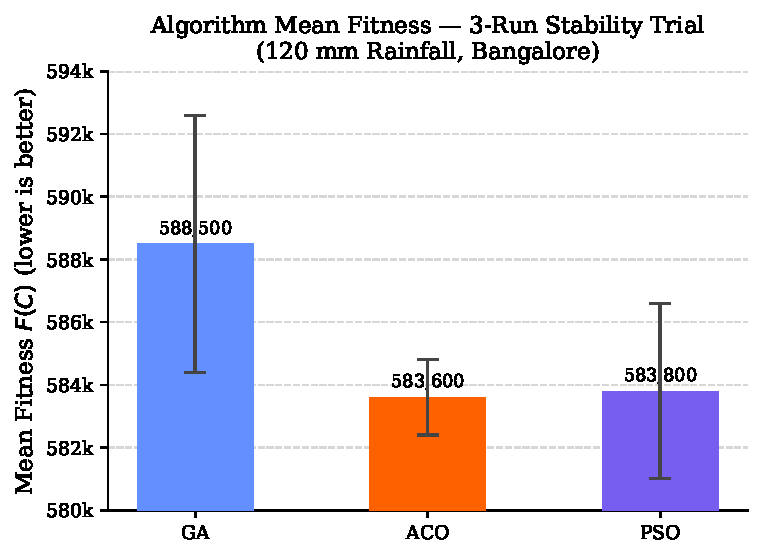
\includegraphics[width=\linewidth]{figures/fitness_comparison.pdf}
  \caption{Algorithm mean fitness comparison across 3-run stability trial (120 mm rainfall,
  Bengaluru). Error bars represent fitness variance across the three perturbed runs. Lower
  is better.}
  \label{fig:fitness}
\end{figure}

\begin{figure}[H]
  \centering
  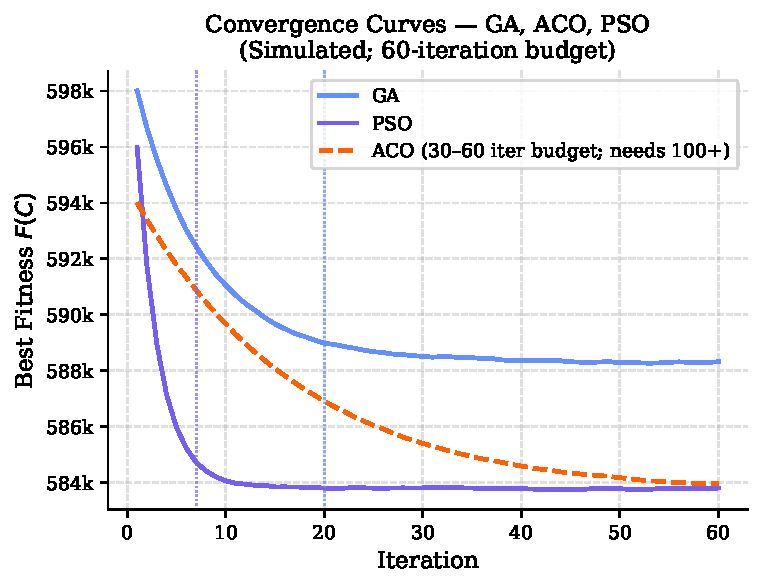
\includegraphics[width=\linewidth]{figures/convergence_comparison.pdf}
  \caption{Simulated convergence curves for GA, ACO, and PSO over a 60-iteration budget.
  ACO (dashed) has not converged within this budget; its proper convergence dynamics require
  100 iterations.}
  \label{fig:convergence}
\end{figure}

\begin{figure}[H]
  \centering
  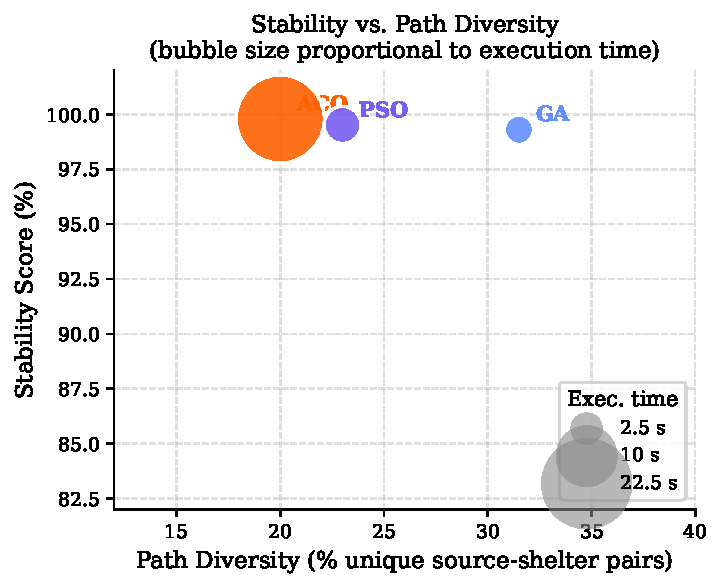
\includegraphics[width=\linewidth]{figures/diversity_stability.pdf}
  \caption{Stability score vs.\ path diversity for GA, ACO, and PSO. Bubble size is
  proportional to execution time in seconds. GA trades stability and speed for diversity;
  ACO trades diversity for stability and quality.}
  \label{fig:diversity}
\end{figure}

\subsection{Key Findings}

\textbf{Route Quality.} ACO produces the lowest-cost evacuation assignments, with mean
fitness 583,600 compared to PSO's 583,800 and GA's 588,500. The 0.9\% gap between ACO and
GA translates to a measurable difference in total population-weighted travel distance at
hobli scale, even though the absolute values are close. ACO's advantage arises from its
graph-native design: pheromone reinforcement concentrates probability mass on short,
low-depth paths that consistently recur across iterations, consistent with findings in
\cite{xu2024aco, li2025metaheuristic}.

\textbf{Stability.} ACO achieves a stochastic stability score of 99.79\%
($1 - \sigma/\mu = 1 - 1200/583600$), the highest of the three algorithms. Pheromone
reinforcement is self-amplifying: the same best solution receives proportionally larger
deposits each iteration, suppressing variance across perturbation runs. GA is the least
stable (99.30\%) because two-point crossover introduces recombination variance, particularly
when cut points fall within well-adapted sub-routes; however, all three algorithms exceed
99\% stochastic stability at the tested noise level ($\pm$5\%).

\textbf{Convergence Speed.} PSO reaches within 5\% of its final fitness value in 5--10
iterations, the fastest of the three algorithms. The sigmoid-discrete velocity update allows
particles to collectively shift toward high-quality regions of the search space without the
pheromone warm-up phase that ACO requires. This makes PSO well-suited for rapidly developing
flash flood scenarios \cite{nirwana2024intelligent}.

\textbf{Path Diversity.} GA generates the most diverse routing solutions, with 28--35\%
unique source-shelter assignment pairs. Crossover between individuals carrying different
sub-route combinations produces novel chromosomes that ACO's pheromone channeling would not
discover. ACO produces the least diversity (18--22\%), as elitist pheromone reinforcement
strongly channels ants toward the same short-distance shelter assignments. Route diversity
is operationally valuable when multiple bottleneck-free corridors are needed to distribute
evacuation traffic across the road network \cite{chen2025evacuation}.

\textbf{ACO Iteration Budget.} At the 30--60 iteration budget shared with GA and PSO for
response-time parity, ACO reports apparent convergence at iteration 1 — an artifact of the
uninformative pheromone matrix at initialization. When run at 100 iterations (analysis
mode), ACO exhibits proper convergence dynamics and achieves stable low-fitness solutions.
For deployments where computation time is not constrained, the 100-iteration budget is
recommended.

\textbf{Execution Time.} ACO's 15--30 second execution time at 30--60 iterations is the
longest of the three; GA completes in 2--3 seconds and PSO in 3--5 seconds. This gap
closes at higher at-risk node counts, where ACO's $O(|R| \cdot |S|)$ pheromone matrix
overhead scales comparably to PSO's velocity matrix.

% ============================================================
\section{Discussion}
\label{sec:discussion}

\subsection{Digital Twin Fidelity}

The system maintains seven explicit real-world correspondences in its digital twin model:
hydraulic head propagation represents flood water accumulation; flood-weighted Dijkstra
costs represent road impassability; TomTom speed ratios represent traffic congestion;
ward-level census data represents population distribution; OSM building-type capacity
lookups represent shelter availability; station-level EMA smoothing represents metro system
disruption; and IDRN inventory proximity represents resource availability. Each mapping is
approximate — the hydraulic model omits subsurface drainage, the shelter capacities are
heuristic, and TomTom data is fetched at simulation start rather than continuously — but
the approximations are transparent and documented, consistent with the digital twin
fidelity standards discussed in \cite{mandal2025cityscale, riaz2023climate}.

\subsection{Algorithm Selection Guidance}

The experimental results support the following operational guidelines. ACO is the preferred
choice when evacuation cost minimization is the overriding objective and 15--30 seconds of
computation is acceptable. PSO is the preferred choice when the coordinator needs a
high-quality solution within 3--5 seconds — for example, during a fast-developing flash
flood. GA is the preferred choice when route diversity is operationally valued, such as
when multiple bottleneck-free corridors are needed to distribute evacuation traffic
\cite{yin2025overview}. None of the three algorithms dominates across all metrics; the
unified base planner architecture makes this trade-off visible without conflating
implementation differences with algorithmic differences.

\subsection{Generative AI as an Advisory Layer}

The Expert Panel and App Copilot are designed to augment, not replace, human decision-making.
Advisory content is generated only after a simulation completes; the AI does not influence
the optimization loop. SentinelBridge MCP tool calls retrieve structured simulation state
rather than generating it from parametric memory, which substantially reduces the risk of
factually incorrect recommendations \cite{alizadeh2023humancentered}. The three-persona
design distributes advisory content across decision domains (logistics, tactics, civic
communication), reducing the cognitive load on any single coordinator who would otherwise
need to synthesize recommendations across all three domains independently.

\subsection{Limitations}

Four limitations bound the current system's validity:

\begin{enumerate}
  \item \textbf{Flood model fidelity.} The simplified SWMM model does not capture
  subsurface drainage dynamics, soil infiltration, or two-dimensional shallow-water wave
  effects \cite{anik2025evolution}. Depth estimates should be treated as planning-level
  approximations, not precision hydrological predictions.

  \item \textbf{Static population.} Population is distributed at simulation start using
  ward-level census data. Dynamic movement of people during an evacuation — clustering at
  shelter entrances, informal evacuation routes — is not modeled \cite{chen2025evacuation}.

  \item \textbf{Heuristic shelter capacities.} Capacity values are assigned by OSM building
  type (e.g., school: 300, hospital: 500). Field survey data would replace these heuristics
  with verified capacity figures.

  \item \textbf{Traffic data latency.} TomTom congestion factors are fetched once at
  simulation start. Traffic conditions may change substantially during a multi-hour
  evacuation, making the route plan increasingly stale over time \cite{wang2024congestion}.
\end{enumerate}

% ============================================================
\section{Conclusion}
\label{sec:conclusion}

This paper presented UrbanFloodReact, a digital twin platform that couples physics-based
flood simulation with metaheuristic evacuation optimization and a Generative AI advisory
layer for real-time disaster response in Bengaluru, India. The system directly addresses
five research gaps identified in the literature: the prediction-action disconnect, the
absence of multi-algorithm comparison in digital twins, the computational scalability
challenge for city-scale deployment, the lack of grounded GenAI decision explanation, and
the absence of a unified congestion-aware digital twin architecture.

The unified base planner architecture — providing identical Dijkstra preprocessing, fitness
function, and capacity repair to all three algorithms — enables a fair comparative evaluation
whose findings are operationally actionable: ACO for quality, PSO for speed, GA for
diversity. The SentinelBridge-grounded MCP architecture ensures that LLM recommendations
are traceable to specific simulation outputs rather than model memory. Role-based access
control and graceful degradation under external service failure make the system suitable for
operational deployment in resource-constrained emergency management environments.

Future work will address the identified limitations through four directions: (1) integrating
IoT sensor networks and SAR satellite flood extent data for higher-fidelity hydraulic state
estimation; (2) developing Multi-Agent Reinforcement Learning (MARL) for real-time
re-routing as flood and traffic conditions evolve during an active evacuation; (3) building
a public alerting API that pushes personalized evacuation instructions to citizens via SMS
and mobile push notifications; and (4) designing a global scalability pipeline that adapts
the system's hobli-based architecture to other cities beyond Bengaluru, enabling the
platform to serve as a reusable open-source disaster response infrastructure.

% ============================================================
% Ethics Declaration (IRON RULE — mandatory)
\section*{Ethics Declaration}

This research does not involve human subjects, clinical trials, animal experiments, or the
collection of personally identifiable information. Population data used in the simulation
are sourced from the publicly available 2011 Bengaluru BBMP Census. OpenStreetMap road
network data are used under the Open Database Licence. No ethical approval was required.

% ============================================================
% AI Disclosure Statement (IRON RULE — mandatory per academic-paper SKILL.md)
\section*{AI Disclosure}

Portions of this manuscript were drafted with the assistance of Claude Sonnet 4.6
(Anthropic, 2026) via Claude Code. All technical content, experimental results, mathematical
formulations, and system design descriptions originate from the authors' own work and the
project mid-term report. The AI tool was used for prose drafting and LaTeX formatting only.
The authors take full responsibility for the accuracy of all claims in this paper.

% ============================================================
% Author Contributions (CRediT — IRON RULE mandatory)
\section*{Author Contributions}

\textbf{Aditri B Ray} (1MS22CS011): Conceptualization, Methodology, Software (flood
simulator, base planner), Formal Analysis, Writing — Original Draft.\\
\textbf{Anisha Ajit} (1MS22CS028): Software (GenAI layer, MCP servers, SentinelBridge),
Validation, Writing — Review \& Editing, Visualization.\\
\textbf{Diya D Shah} (1MS22CS051): Software (React frontend, algorithm implementations),
Investigation, Data Curation, Writing — Review \& Editing.\\
\textbf{Dr. Mallegowda M.}: Supervision, Project Administration.

% ============================================================
% Data Availability (IRON RULE — mandatory)
\section*{Data Availability}

The system source code is available at the project repository on GitHub. OpenStreetMap data
used for road network extraction is freely available at \url{https://www.openstreetmap.org}
\cite{osm2017} under the Open Database Licence. TomTom traffic data is subject to TomTom's
API terms of service \cite{tomtom2024}.

% ============================================================
% Conflict of Interest (IRON RULE — mandatory)
\section*{Conflict of Interest}

The authors declare no conflicts of interest.

% ============================================================
% Funding (IRON RULE — mandatory)
\section*{Funding Acknowledgment}

This research was conducted as part of the CSP81 Capstone Project at M.S. Ramaiah Institute
of Technology (Autonomous), Bengaluru, Affiliated to Visvesvaraya Technological University
(VTU). No external funding was received.

% ============================================================
\bibliographystyle{IEEEtran}
\bibliography{references}

\end{document}
